\documentclass[12pt]{beamer}
\usetheme{Pittsburgh}
\usepackage[utf8]{inputenc}
\usepackage[english]{babel}
\usepackage{amsmath}
\usepackage{amsfonts}
\usepackage{amssymb}
\usepackage{graphicx}
\author{Sebastian Valet, Johannes Walter}
\title{Human Capital Investments and Expectations about Career and Family}
%\setbeamercovered{transparent} 
%\setbeamertemplate{navigation symbols}{} 
%\logo{} 
%\institute{} 
%\date{} 
%\subject{} 
\begin{document}

\begin{frame}
\titlepage
\end{frame}

%\begin{frame}
%\tableofcontents
%\end{frame}

% These sildes can probably go in the appendix
\begin{frame}{Current Population Characteristics I}
    \begin{itemize}
        \item Earnings, employment, and marriage data  for the US population using the 2009
        \item Not suited for causal inference; needs not reflect the student's beliefs
        \item Data from older cohort; includes not only high-ability participants
        \item But data is suited to document that career and family outcomes differ by educational choices in observational data
    \end{itemize}
\end{frame}

\begin{frame}{Current Population Characteristics II}
    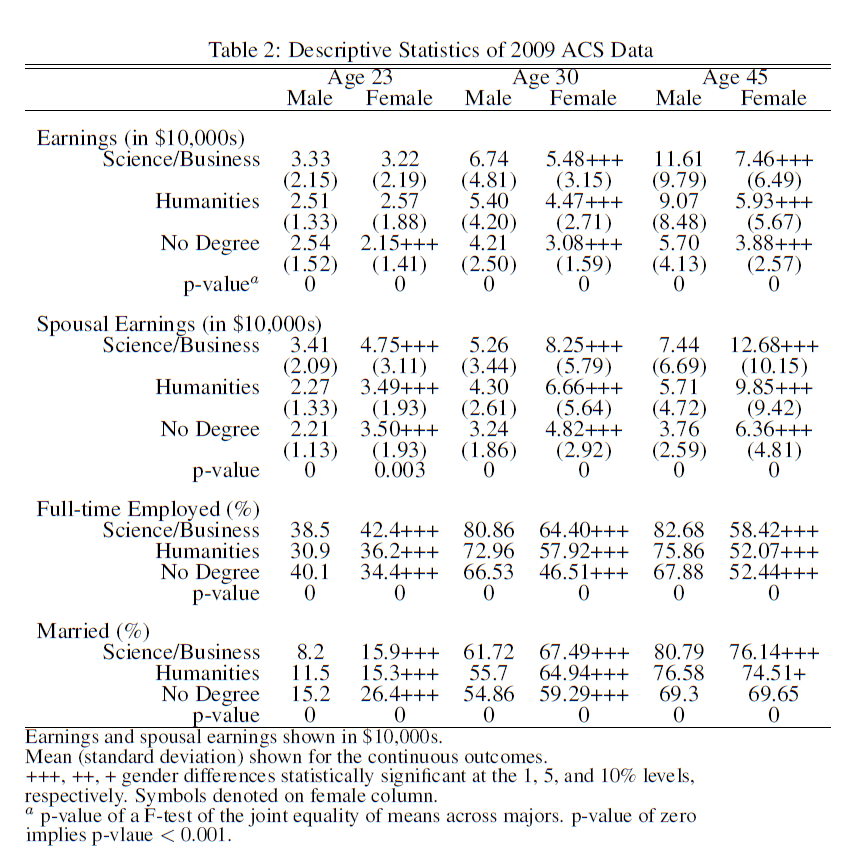
\includegraphics[scale=0.4]{Table2.png}
\end{frame}

% Earnings Beliefs: Earnings Levels
\begin{frame}{Earnings Beliefs: Earnings Levels}
    \begin{itemize}
        \item male students believe to earn more than female students at each age
        \item all students believe to see rapid growth in earnings
        \item students believe to see substantially smaller earning growth if they don't major in science/business
        \item Perceived gender gap is largest in science/business and at later stages

       \end{itemize}
\end{frame}

\begin{frame}{Earnings Beliefs: Earnings Levels}
    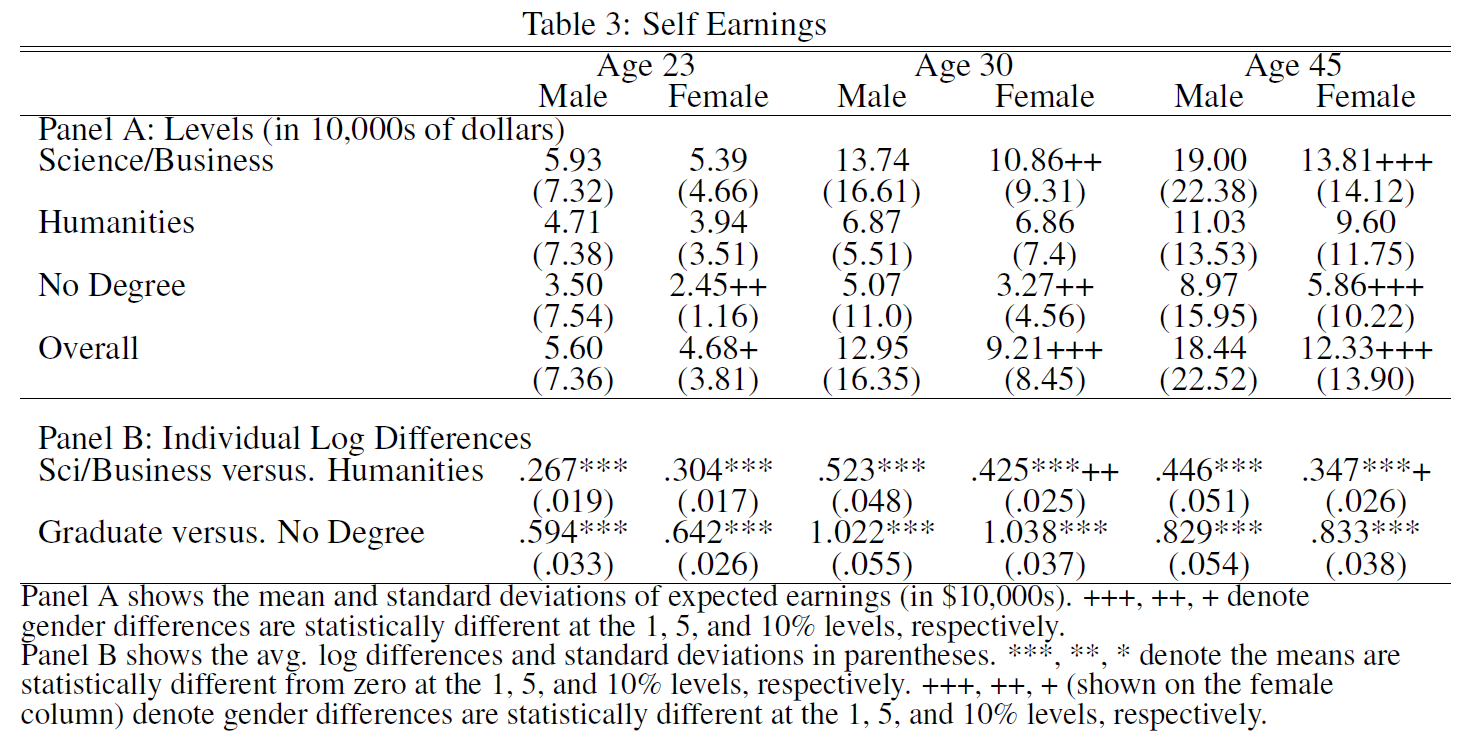
\includegraphics[scale=0.35]{Graphs/Table 3 Self Earnings.png}
\end{frame}

% Earnings Beliefs: Earnings Growth
\begin{frame}{Earnings Growth}
    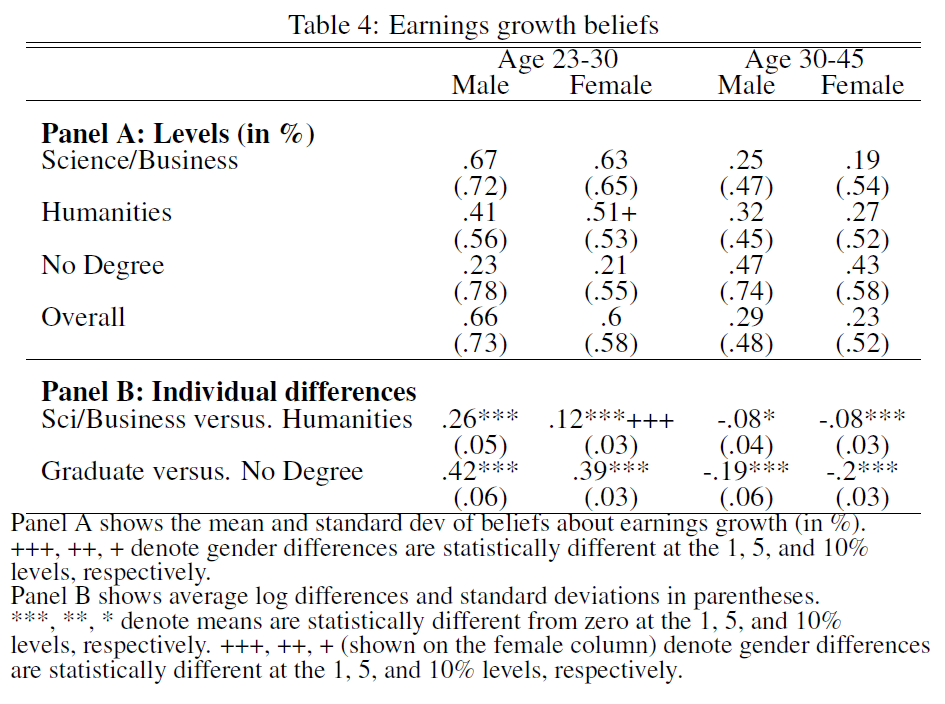
\includegraphics[scale=0.35]{Graphs/Table 4 Earnings Growth Belief.png}
\end{frame}

% Earnings Beliefs: Earnings Uncertainty
\begin{frame}{Earnings Uncertainty}
    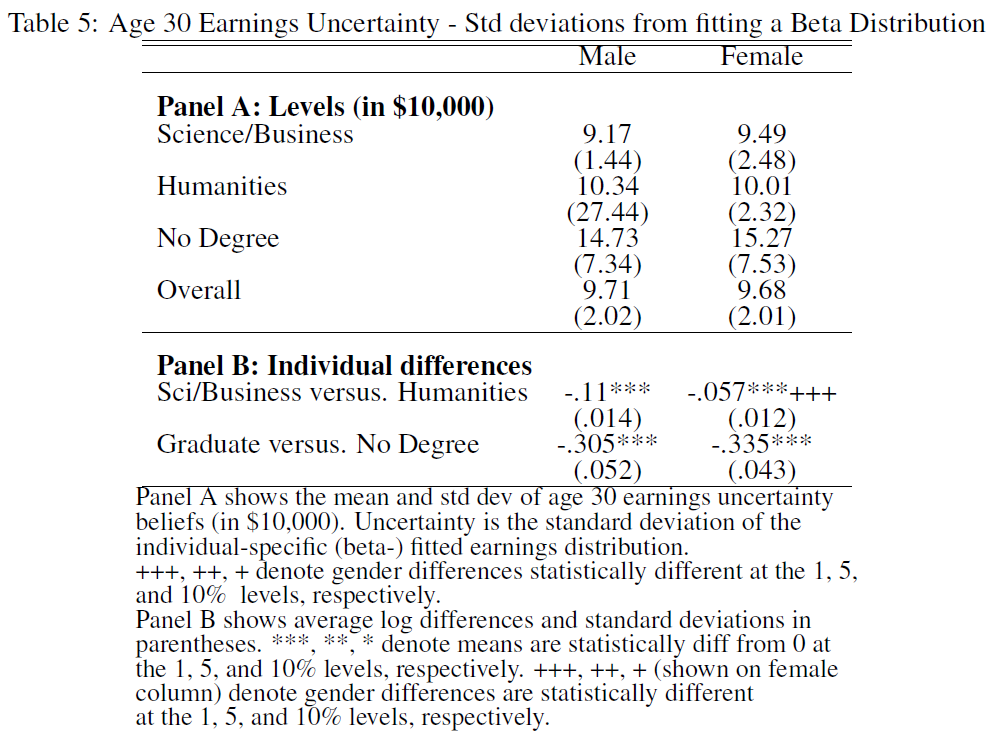
\includegraphics[scale=0.35]{Graphs/Table 5 Age 30 Earnings Uncertainty.png}
\end{frame}

% Beliefs about Marriage
\begin{frame}{Beliefs about Marriage}
    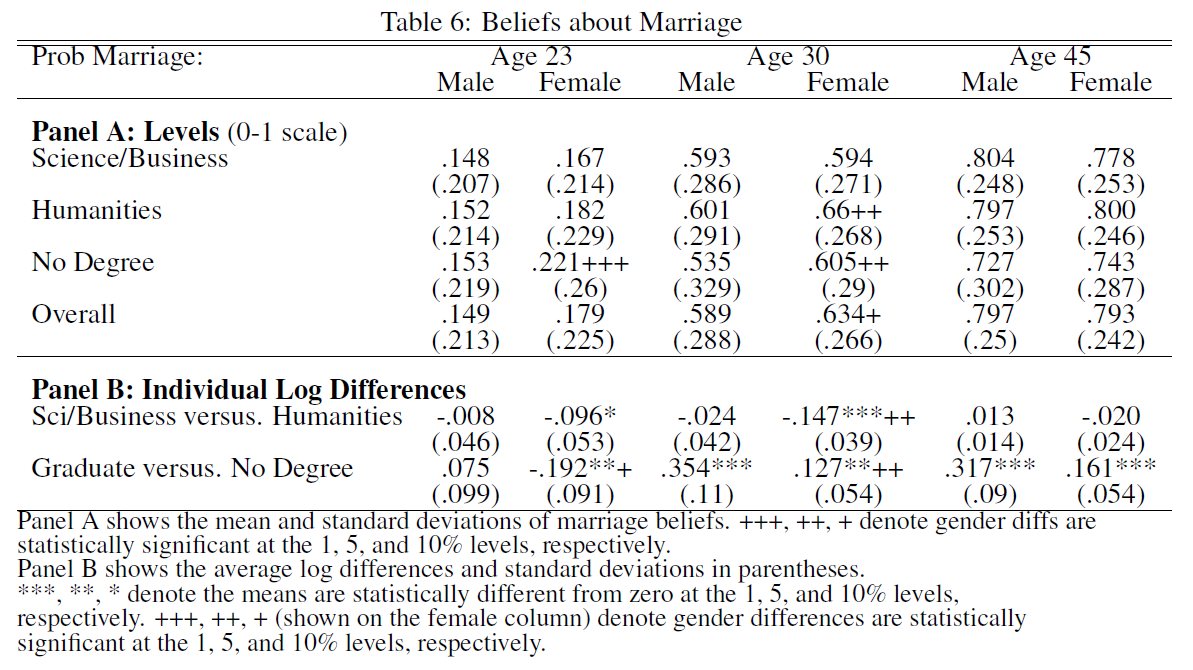
\includegraphics[scale=0.35]{Graphs/Table 6 Beliefs about Marriage.png}
\end{frame}

% Beliefs about Potential Spousal Earnings
\begin{frame}{Beliefs about Potential Spousal Earnings}
    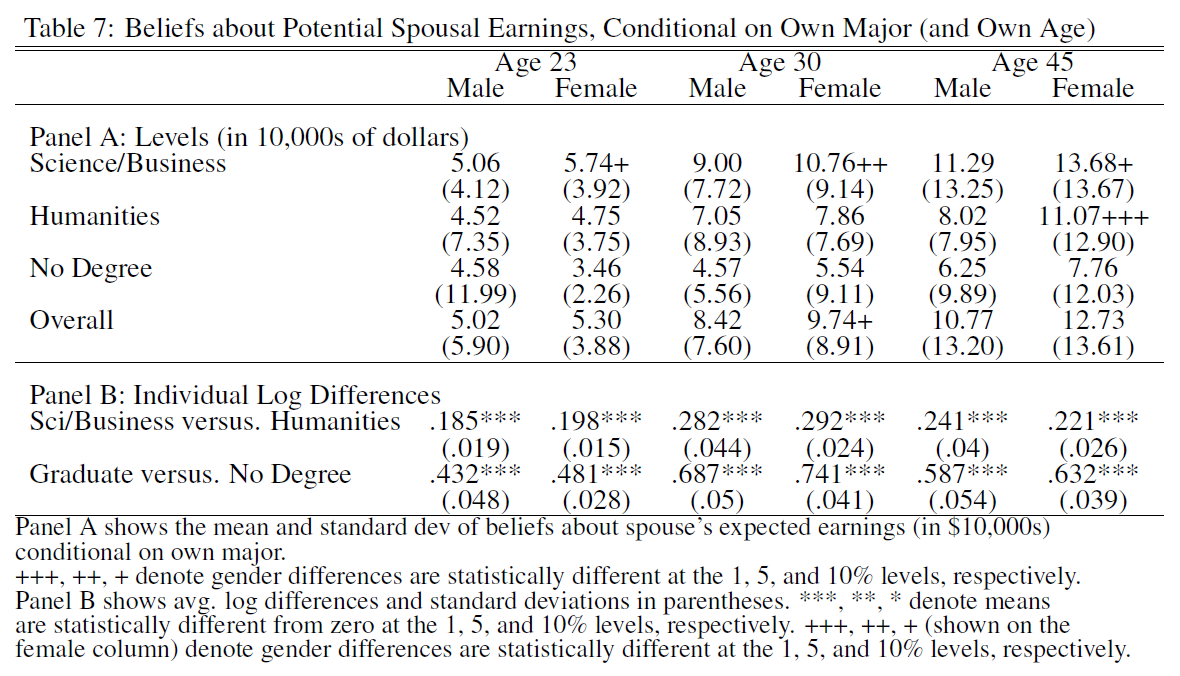
\includegraphics[scale=0.35]{Graphs/Table 7 Beliefs about Potential Spousal Earnings.png}
\end{frame}

\end{document}